%% BioMed_Central_Tex_Template_v1.06
%%                                      %
%  bmc_article.tex            ver: 1.06 %
%                                       %

%%IMPORTANT: do not delete the first line of this template
%%It must be present to enable the BMC Submission system to
%%recognise this template!!

%%%%%%%%%%%%%%%%%%%%%%%%%%%%%%%%%%%%%%%%%
%%                                     %%
%%  LaTeX template for BioMed Central  %%
%%     journal article submissions     %%
%%                                     %%
%%          <8 June 2012>              %%
%%                                     %%
%%                                     %%
%%%%%%%%%%%%%%%%%%%%%%%%%%%%%%%%%%%%%%%%%


%%%%%%%%%%%%%%%%%%%%%%%%%%%%%%%%%%%%%%%%%%%%%%%%%%%%%%%%%%%%%%%%%%%%%
%%                                                                 %%
%% For instructions on how to fill out this Tex template           %%
%% document please refer to Readme.html and the instructions for   %%
%% authors page on the biomed central website                      %%
%% http://www.biomedcentral.com/info/authors/                      %%
%%                                                                 %%
%% Please do not use \input{...} to include other tex files.       %%
%% Submit your LaTeX manuscript as one .tex document.              %%
%%                                                                 %%
%% All additional figures and files should be attached             %%
%% separately and not embedded in the \TeX\ document itself.       %%
%%                                                                 %%
%% BioMed Central currently use the MikTex distribution of         %%
%% TeX for Windows) of TeX and LaTeX.  This is available from      %%
%% http://www.miktex.org                                           %%
%%                                                                 %%
%%%%%%%%%%%%%%%%%%%%%%%%%%%%%%%%%%%%%%%%%%%%%%%%%%%%%%%%%%%%%%%%%%%%%

%%% additional documentclass options:
%  [doublespacing]
%  [linenumbers]   - put the line numbers on margins

%%% loading packages, author definitions

%\documentclass[twocolumn]{bmcart}% uncomment this for twocolumn layout and comment line below
\documentclass{bmcart}

%%% Load packages
%\usepackage{amsthm,amsmath}
%\RequirePackage{natbib}
%\RequirePackage[authoryear]{natbib}% uncomment this for author-year bibliography
%\RequirePackage{hyperref}
\PassOptionsToPackage{hyphens}{url}\usepackage{hyperref}
\usepackage[utf8]{inputenc} %unicode support
%\usepackage[applemac]{inputenc} %applemac support if unicode package fails
%\usepackage[latin1]{inputenc} %UNIX support if unicode package fails


%%%%%%%%%%%%%%%%%%%%%%%%%%%%%%%%%%%%%%%%%%%%%%%%%
%%                                             %%
%%  If you wish to display your graphics for   %%
%%  your own use using includegraphic or       %%
%%  includegraphics, then comment out the      %%
%%  following two lines of code.               %%
%%  NB: These line *must* be included when     %%
%%  submitting to BMC.                         %%
%%  All figure files must be submitted as      %%
%%  separate graphics through the BMC          %%
%%  submission process, not included in the    %%
%%  submitted article.                         %%
%%                                             %%
%%%%%%%%%%%%%%%%%%%%%%%%%%%%%%%%%%%%%%%%%%%%%%%%%


%\def\includegraphic{}
%\def\includegraphics{}
\usepackage{graphicx}


%%% Put your definitions there:
\startlocaldefs
\endlocaldefs

\newcommand{\variantSpark}{{\sc VariantSpark}}
\newcommand{\kMeans}{\textit{k}-means}
\newcommand{\ARI}{adjusted Rand index}


%%% Begin ...
\begin{document}

%%% Start of article front matter
\begin{frontmatter}

\begin{fmbox}
\dochead{Research}

%%%%%%%%%%%%%%%%%%%%%%%%%%%%%%%%%%%%%%%%%%%%%%
%%                                          %%
%% Enter the title of your article here     %%
%%                                          %%
%%%%%%%%%%%%%%%%%%%%%%%%%%%%%%%%%%%%%%%%%%%%%%

\title{VariantSpark: Population Scale Clustering of Genotype Information}

%%%%%%%%%%%%%%%%%%%%%%%%%%%%%%%%%%%%%%%%%%%%%%
%%                                          %%
%% Enter the authors here                   %%
%%                                          %%
%% Specify information, if available,       %%
%% in the form:                             %%
%%   <key>={<id1>,<id2>}                    %%
%%   <key>=                                 %%
%% Comment or delete the keys which are     %%
%% not used. Repeat \author command as much %%
%% as required.                             %%
%%                                          %%
%%%%%%%%%%%%%%%%%%%%%%%%%%%%%%%%%%%%%%%%%%%%%%

\author[
   addressref={aff1,aff2},                   % id's of addresses, e.g. {aff1,aff2}
%   corref={aff1},                       % id of corresponding address, if any
%   noteref={n1},                        % id's of article notes, if any
%   email={jane.e.doe@cambridge.co.uk}   % email address
]{\inits{}\fnm{Aidan R.} \snm{O'Brien}}
\author[
   addressref={aff1},
]{\inits{}\fnm{Neil} \snm{Saunders}}
\author[
   addressref={aff3,aff4},
%   email={john.RS.Smith@cambridge.co.uk}
]{\inits{}\fnm{Fabian A.} \snm{Buske}}
\author[
   addressref={aff1},
   email={Denis.Bauer@CSIRO.au}
%   email={john.RS.Smith@cambridge.co.uk}
]{\inits{}\fnm{Denis C.} \snm{Bauer}}
%%%%%%%%%%%%%%%%%%%%%%%%%%%%%%%%%%%%%%%%%%%%%%
%%                                          %%
%% Enter the authors' addresses here        %%
%%                                          %%
%% Repeat \address commands as much as      %%
%% required.                                %%
%%                                          %%
%%%%%%%%%%%%%%%%%%%%%%%%%%%%%%%%%%%%%%%%%%%%%%

\address[id=aff1]{%                           % unique id
  \orgname{CSIRO, Health \& Biosecurity Flagship}, % university, etc
  \street{11 Julius Av},                     %
  \postcode{2113},                                % post or zip code
  \city{Sydney},                              % city
  \cny{Australia}                                    % country
}
\address[id=aff2]{%
  \orgname{School of Biomedical Sciences and Pharmacy, Faculty of Health},
  \postcode{2308},
  \city{Newcastle},
  \cny{Australia}
}
\address[id=aff3]{%
  \orgname{Cancer Epigenetics Program, Cancer Research Division, Kinghorn Cancer Centre, Garvan Institute of Medical Research},
  \street{384 Victoria St},
  \postcode{2010},
  \city{Sydney},
  \cny{Australia}
}
\address[id=aff4]{%
  \orgname{UNSW Medicine, University of New South Wales},
%  \street{384 Victoria St},
  \postcode{2052},
  \city{Sydney},
  \cny{Australia}
}
%%%%%%%%%%%%%%%%%%%%%%%%%%%%%%%%%%%%%%%%%%%%%%
%%                                          %%
%% Enter short notes here                   %%
%%                                          %%
%% Short notes will be after addresses      %%
%% on first page.                           %%
%%                                          %%
%%%%%%%%%%%%%%%%%%%%%%%%%%%%%%%%%%%%%%%%%%%%%%

\begin{artnotes}
%\note{Sample of title note}     % note to the article
\note[id=n1]{Equal contributor} % note, connected to author
\end{artnotes}

\end{fmbox}% comment this for two column layout

%%%%%%%%%%%%%%%%%%%%%%%%%%%%%%%%%%%%%%%%%%%%%%
%%                                          %%
%% The Abstract begins here                 %%
%%                                          %%
%% Please refer to the Instructions for     %%
%% authors on http://www.biomedcentral.com  %%
%% and include the section headings         %%
%% accordingly for your article type.       %%
%%                                          %%
%%%%%%%%%%%%%%%%%%%%%%%%%%%%%%%%%%%%%%%%%%%%%%

\begin{abstractbox}

\begin{abstract} % abstract
\parttitle{Motivation} Genomic information is increasingly used in medical practice, giving rise to the need for efficient analysis methodology able to cope with thousands of individuals and millions of variants. The widely used Hadoop MapReduce architecture and associated machine learning library, Mahout, provide the means for tackling computationally challenging tasks. However, many genomic analyses do not fit the Map-Reduce paradigm. We therefore survey the recently developed {\sc Spark} engine, along with its associated machine learning library, MLlib, which are more flexible in the parallelisation architecture and hence more suitable for population-scale bioinformatics tasks. To do this, we developed an interface from Mahout and MLlib to the standard variant format (VCF), which opens up the usage of advanced, efficient machine learning algorithms to genomic data. 

\parttitle{Results} We successfully clustered more than 2,500 individuals each having more than 38 Million variants. Both Hadoop and {\sc Spark} have superior performance over traditional approaches. We observe a 50 fold speedup when using the efficient in-memory {\sc Spark} compute engine compared to Hadoop. Furthermore, our implementation achieves a better performance compared to a previously published {\sc Spark}-based genome clustering approach, {\sc ADAM}.

\parttitle{Availability} The package is written in Scala and available at \url{https://github.com/BauerLab/VariantSpark}.
\end{abstract}

%%%%%%%%%%%%%%%%%%%%%%%%%%%%%%%%%%%%%%%%%%%%%%
%%                                          %%
%% The keywords begin here                  %%
%%                                          %%
%% Put each keyword in separate \kwd{}.     %%
%%                                          %%
%%%%%%%%%%%%%%%%%%%%%%%%%%%%%%%%%%%%%%%%%%%%%%

\begin{keyword}
\kwd{sample}
\kwd{article}
\kwd{author}
\end{keyword}

% MSC classifications codes, if any
%\begin{keyword}[class=AMS]
%\kwd[Primary ]{}
%\kwd{}
%\kwd[; secondary ]{}
%\end{keyword}

\end{abstractbox}
%
%\end{fmbox}% uncomment this for twcolumn layout

\end{frontmatter}

%%%%%%%%%%%%%%%%%%%%%%%%%%%%%%%%%%%%%%%%%%%%%%
%%                                          %%
%% The Main Body begins here                %%
%%                                          %%
%% Please refer to the instructions for     %%
%% authors on:                              %%
%% http://www.biomedcentral.com/info/authors%%
%% and include the section headings         %%
%% accordingly for your article type.       %%
%%                                          %%
%% See the Results and Discussion section   %%
%% for details on how to create sub-sections%%
%%                                          %%
%% use \cite{...} to cite references        %%
%%  \cite{koon} and                         %%
%%  \cite{oreg,khar,zvai,xjon,schn,pond}    %%
%%  \nocite{smith,marg,hunn,advi,koha,mouse}%%
%%                                          %%
%%%%%%%%%%%%%%%%%%%%%%%%%%%%%%%%%%%%%%%%%%%%%%

%%%%%%%%%%%%%%%%%%%%%%%%% start of article main body
% <put your article body there>

%%%%%%%%%%%%%%%%
%% Background %%
%%
\section*{Background}

Genomic information is increasingly used in medical practice.
A commonly performed task in such applications is grouping individuals based on their genomic profile to identify population association~\cite{Gao2007} or elucidate different haplotype involvement in diseases susceptibility~\cite{Laitman2013}.  
The commonly used tool is {\sc Admixture}~\cite{Alexander2009}, which performs maximum likelihood estimation of individual ancestries from multilocus SNP genotype datasets.
Due to the decreasing sequencing cost it is economical to generate studies with sample sizes previously reserved for larger consortia such as the 1000 Genomes Project~\cite{1KG2012} or The Cancer Genome Atlas, TCGA~\cite{TCGA2013}. 
At the same time, whole genome sequencing enables the inclusion of rare or even somatic mutations in the analysis, increasing the feature space by orders of magnitude. This drastic increase in both sample numbers and features per sample requires a massively parallel approach to data processing~\cite{Stein2010}. Traditional parallelisation strategies like OpenMPI or hardware accelerators (GPGPU) cannot scale with variable data sizes or require purpose-built hardware.
 
Addressing this issue, {\sc Apache Hadoop MapReduce}~\cite{Borthakur2007} transforms data into `key-value pairs' that can then be distributed between multiple nodes across a commodity computer cluster, depending on the size of the problem. 
MapReduce approaches are increasingly being used in bioinformatics (for reviews see~\cite{Zou2013, Qiu2010,Taylor2010}). 
This is especially the case for sequence analysis tasks, such as read mapping~\cite{Schatz2009}, duplicate removal~\cite{Jourdren2012}, and variant calling~\cite{Langmead2009, McKenna2010} as well as Genome Wide Analysis Study based tasks~\cite{Huang2013, Guo2014}. 
Apache also developed a machine learning library, Mahout~\cite{Owen2011}, which allows efficient out-of-the-box analysis to be applied to clinical applications, such as medical health records~\cite{Ko2014}.
Unfortunately, the MapReduce paradigm is not always the optimal solution, specifically for bioinformatics or machine learning applications that require iterative in-memory computation. Specifically, Hadoop is disk IO intensive, and this can prove to be a bottleneck in processing-speed.

{\sc Apache Spark}~\cite{Zaharia2011} is a more recent compute engine, which overcomes many of Hadoop's limitations. 
One of the main benefits is that it allows programs to cache data in memory; potentially eliminating, or at least reducing, the bottleneck of disk IO. 
When utilising caching, Apache claim {\sc Spark} to be 100x faster than Hadoop. 
Although {\sc Spark} allows MapReduce-like programs, it does not require programs to exactly model the MapReduce paradigm, which in turn allows more flexibility when designing programs. 
Recognising the capability, the Big Data Genomics (BDG) group recently demonstrated the strength of {\sc Spark} in a genomic clustering application using {\sc ADAM}, a set of formats and APIs as well as processing stage implementations for genomic data~\cite{Massie2013}. 
While the speedup over traditional methods was impressive (50 fold speedup), being limited by constraints within this general genomics framework hampered performance. 

We hence developed a more focused purpose-built application in {\sc Spark} to perform genomic clustering of individuals. 
We utilise {\sc Spark}'s machine learning library, \mbox{MLlib}, and provide an interface to the standard variant data format, Variant Call Format (VCF)~\cite{1KG2012}, which opens up the application of MLlib's different machine learning algorithms to a wide range of genotype-based analysis tasks. 

To demonstrate \variantSpark's capability, we cluster variant datasets from the 1000 Genomes Project~\cite{1KG2012} to determine population structure using the \kMeans{} clustering algorithm available in MLlib. 
In the first section we benchmark \variantSpark's performance and accuracy against {\sc ADAM} and a Hadoop Mahout implementation as well as more traditional methods (R, Python) and the purpose-build tool {\sc Admixture}~\cite{Alexander2009} limiting the used data to chromosome 22.
In section two we demonstrate \variantSpark's full capacity by seamlessly scaling from 20\% to 100\% of the human genome.
In section three we replicate the analysis by using 478 genomes from the Personal Genome Project~\cite{Lunshof2013}.
In the last section we discuss the pipeline for visualising the resulting cluster. 


\section*{Results and discussions}

\subsection*{{\sc Spark} enables faster clustering of individuals compared to traditional methods}

In this section we compare the time required to cluster individuals based on genomic variants using \variantSpark{} against {\sc ADAM} as well as the more traditional approaches using Hadoop (and Mahout), Python and R. 
We limit the genomic variants to only chromosome 22 as the traditional approaches have substantially larger memory consumption, rendering a whole-genome input infeasible.  
Furthermore, we perform the comparisons on a single virtual machine to ensure the six different approaches have access to the same resources.
We use \kMeans{} clustering algorithms in the respective implementations, which require the VCF input files to be pre-processed (see methods). 
The state-of-the-art tool, {\sc Admixture}, also requires a pre-processing step from VCF to PED format, which we performed using GAKT~\cite{McKenna2010}.
We therefore compare the time required for the pre-processing step, as well as for \kMeans{} clustering.

As shown in Table 1, pre-processing the data is fastest in \variantSpark{}, requiring 2mins and 58secs. %178s 
This is almost 80\% faster than the {\sc ADAM} implementation (12min and 48secs) %768s
or our Hadoop implementation (14min and 22secs), respectively. %862s
Unlike \variantSpark{} and our Hadoop implementation, the {\sc ADAM} framework cannot process the VCF files directly but requires them to be converted into a binary {\sc ADAM} file format. 
Although this additional pre-processing step is only required once for each input file, it requires an additional 13mins and 13secs, %793s
rendering our approach almost an order of magnitude faster (see Figure 1).
R and Python are also slower at pre-processing, taking 67 minutes and 92 minutes, respectively. 
This increased pre-processing time is due to the Python and R implementations not natively supporting multithreading, while \variantSpark{}, {\sc ADAM} and Hadoop can use the eight available cores.
The GATK-based VCF to PED conversion is also slower with over 10 minutes. 

Clustering the samples is also fastest in \variantSpark{} (1min and 20secs, see Table 1), despite \variantSpark{} and {\sc ADAM} both using {\sc Spark}'s MLlib \kMeans{} implementation. % 80
% DENIS: how sure are we that this is not just a fluke, e.g. I typically repeat this 5 times and report the average and std/ste ...
% AIDAN: This result was consistent. But it was on the Azure cluster so I can't get std/ste..
% DENIS: OK but I thought all of them were run on the same machine and you are still generating results for python ... 
% TODO:  write something like (repeated X times)
We attribute the 30\% speedup over {\sc ADAM} (1min and 52secs) to \variantSpark{} converting the VCF files to sparse vectors, whereas {\sc ADAM} creates dense vectors, which are less memory efficient. %
Multithreading \kMeans{} clustering is natively supported by both R and Python, we are therefore able to utilise eight cores. 
Despite this, both are an order of magnitude slower than \variantSpark{} and {\sc ADAM}, with Python requiring 11mins and 29secs and R requiring 7mins and 25secs.
{\sc Admixture} is also slower with a runtime of just over 8 minutes. 
Our Hadoop implementation performs the worst with 14mins and 23secs, showcasing the limitations of the Hadoop engine. % 863
The substantially increased runtime is due to the dataset (chromosome 22) being small enough to fit into memory, which enables Python and R to store the output from each \kMeans{} iteration in memory. 
Hadoop, however, writes the entire output of each iteration to disk.
Although this Hadoop feature allows for greater scalability, as disk IO is not the run-time determining factor for larger datasets, it introduces a bottleneck for smaller datasets.
{\sc Spark} overcomes this limitation by performing in-memory caching of datasets, which eliminates the disk IO bottleneck on smaller datasets, and minimises the bottleneck on larger datasets where at least a portion of the data can be cached in memory.

We also investigate the cluster quality for the five different methods by comparing the annotated super-population label (AMR, AFR, EAS, SAS) for each individual in the 1000 Genomes data to the assigned label from the clustering allowing four clusters. 
For this comparison, we use the \ARI{} (ARI) metric, which returns a value between -1 (independent labelings) and 1 (perfect match)~\cite{Hubert1985}.
Using chromosome 22, each of the algorithms resulted in an ARI of 0.84, confirming that the speed-up in {\sc Spark} is not at the cost of quality.
Even the state-of-the-art tool, {\sc Admixture} does returns a low ARI=0.25.
We can substantially improve the accuracy to a perfect classification (ARI=1.0) by removing the fourth super-population, AMR (American). 
Including AMR individuals, we observe that the majority of these individuals are placed in the same group as Europeans, likely accurately reflecting their migrational backgrounds. 
Only a minority of AMR individuals form an independent group, likely comprising of genetic information otherwise not captured by the 26 sub-populations of the 1000 genomes project.
This indicates that although allelic differences exist between populations, "genetic diversity is distributed on a continuum"~\cite{Hunter2014}.

\subsection*{\variantSpark{} allows genome wide sampling of variants to improve clustering quality}

Although we have demonstrated the advantages of \variantSpark{} over traditional methods on small datasets, the main advantage of {\sc Spark} is its ability to process datasets that exceed memory limits.
To demonstrate this scalability, we increase the number of variants used in the clustering from the initial 494,328 on chromosome 22 to 38,219,238 including all variants in the genome.

We run this comparison on our in-house Hadoop cluster using 40 cores.
Pre-processing the VCF files takes approximately 12 minutes, 19 minutes, 27 minutes and 40 minutes for 20\%, 40\%, 60\% and 100\% of the genome, respectively (see Table 2).
In each case, the memory required does not exceed a modest 2GB per executor, even for 100\% of the genome. 
Clustering the data takes 70 minutes, 139 minutes, 213 minutes and 884 mins, respectively.
For clustering, the memory requirements increase approximately linearly to 24GB per executor (see Figure 1). 
%This substantial increase in memory required is a result of the increased dimensionality of the data causing the \kMeans{} centroids, which MLlib stores as dense vectors, requiring excessive memory.  
% DENIS: This conflicts with the 30 seconds gain over {\sc ADAM} which you attribute to our clustering using sparse vectors,
% AIDAN: Only centroids are dense. Reworded to explain this
% DENIS: That means you allow more clusters ?
The increase in memory is a result of more \kMeans{} centroids being created, which MLlib stores as dense vectors. 
While \kMeans{} clustering can scale to 100\% of the genome, machine learning algorithms that can deal with sparse vectors would potentially be able to scale much further, for example process more alleles.

%DENIS: do you see a change in ARI from chr22 to 20%, 40% ?
%AIDAN: not really.. 
%DENIS: so it is still exactly 0.84? Can you provide the number of Variants used in the different sets (e.g. is 20\% less than chrom 22)
%TODO A citation would be good here
We do not observe an increase in cluster accuracy when providing variants from other chromosomes, indicating that current practice of clustering based on a subset of the genome is sufficient to define the population boundaries~\cite{Hunter2014}.


\subsection*{Personal Genome Project}
To demonstrate the versatility of \variantSpark{} we also process and cluster individuals from the Personal Genomics Project (PGP). The PGP is open to the public for individuals to submit their genomic sequence along with any metadata, such as diseases or clinical features~\cite{Lunshof2013}. 
We obtain and curate the data (see methods) resulting in 985,790 variants from 478 individuals.

We cluster the individuals allowing five clusters and compare the assigned labels to the same number of self-reported `Race/ethnicity' labels (`White', `Hispanic or Latino', `Asian', `Black or African American' and `American Indian').
The observed ARI is negative, indicating the clustering is random. 
This poor result may be due to the labels being too broad and not accurately reflecting genetic diversity. For example, the `White' label includes individuals with grandparents from United States, Syria, Arab Republic, or Bulgaria, amongst others. 
The dataset is also very one-sided with 433 out of the 478 (over 90\%) of the individuals being classified as white, even though geographical location of their grandparents are very diverse.
% TODO provide mapping
We therefore only include individuals where all grandparents were reported to be from the same country leaving 36 individuals from 23 different countries, which we group into their approximate super-populations (see Supplemental Table X). 
Clustering these individuals results in an ARI of 0.29. 

Although we see an increase in cluster-accuracy when removing individuals with a mixed background and operating at super-population level, the clustering is not as precise as on the carefully curated and characterised individuals from the 1000 Genomes Project.
%TODO add numbers
This is especially the case since XX\% are `White' Americans, which formed the group most difficult to cluster in the 1000 Genomes Project data.

This highlights the issue for clinical application where ancestry influences treatment (e.g. HLA allele genotyping from SNP information~\cite{Zheng2014}) and accurate population association may not be known for patients with diverse migrational background.
Hence fast genome-wide applicable approaches may help in providing the necessary depth to provide insight into genetic diversity. 
% DENIS: statement about why we cannot do more with this data...
Unfortunately, this hypothesis could no not be tested as whole genome information is not available for these individuals. 


\subsection*{Graph visualization}
Add the image here \ldots




\section*{Conclusions}

\variantSpark{} performs clustering on VCF files with over 1000 individuals and 40 Million variants in under 15 hours using minimal memory (24GB). 
\variantSpark{} supports random genome-wide sampling of variants allowing faster clustering for well characterised cohorts where 20\% of the genome is sufficient. 
On the benchmarking dataset, it outperforms {\sc ADAM} by almost an order of magnitude (4 vs 28 minutes) by processing VCF files directly and storing the information in sparse vectors. % 258 vs 1673 
\variantSpark{} utilises {\sc Spark}, which allows for in-memory caching and hence performs 85\% faster than Hadoop (29 min).
This novel parallelization approach is also faster than traditional multithreading with 94\% speedup over R (75 min), and 95\% over Python (103 min).
\variantSpark{} is also superior in performance and accuracy over the current state-of-the-art tool for individual ancestries determination, {\sc Admixture}.
These benefits of speed, resource consumption and scalability demonstrate \variantSpark{} to be the interface for applying other machine learning tools from MlLib to genomic data. 




\section*{Materials and methods}
\subsection*{Computational resources}
We completed the Chromosome 22 comparisons on a virtual machine (VM) hosted on Microsoft Azure. This VM is an A7 Linux instance with 8 cores, 56GB memory and Ubuntu as the OS. 
For the whole-genome clustering, we used our in-house Hadoop cluster. This uses Hadoop 2.5.0, managed by CDH 5. We use Spark 1.3.1. This 13 node cluster has a total of 416 cores and 1.22TB memory.


\subsection*{Datasets}
We used  phase 1 variants from the 1000 Genomes Project. On the 22 autosomes, this dataset contains variants for 1092 individuals, spread over a total 38,219,238 alleles.
We also used a subset of this dataset, the variants from chromosome 22, and this contains 494,328 alleles.
These individuals from these datasets are distributed across four super populations, African (AFR), Mixed American (AMR), East Asian (EAS) and European (EUR).


\subsection*{VariantSpark Implementation}
For each of the implementations, we pre-process the VCF files to arrays of features.
In \variantSpark{} we read in the VCF files as text files to a Resilient Data Set (RDD). RDDs allow us to process the files, line-by-line, in parallel. We parse each line as tab-separated values, and `zip' each value with it's heading from the VCF file.
The key-value pairs (KVPs) from each line in the VCF file are stored in separate arrays. We then `zip' each array with a unique index, where these indexes form identifiers for the alleles.
At this point, we have one array for each line from the VCF file. The values in the arrays are KVPs of the parsed tab-separated values zipped with their heading (individual ID), and each array has a unique index.
We now use a `flatMap' to convert these indexed arrays of KVPs into a less convoluted data-structure, as well as to filter out KVPs that aren't alleles (i.e. KVPs that are VCF metadata).
This results in KVPs where the key is the individual ID, and the value is a tuple of the allele and it's index. We effectively have one KVP for each allele from the VCF file. At this point, each allele is still a string straight from the VCF file (i.e. `0\textbar{}1'), however, we require doubles for MLlib.
To convert this to a double, we take the Hamming distance of the allele, where a 1 represents a heterozygous variant, 2 a homozygous variant, and 0, no variant. Also, for each individual, we filter out any alleles that have no variant, leaving us with KVPs of variants (homozygous and heterozygous) only.
We can now group these KVPs by their key (the individual ID) and map them to sparse vectors. This results in a sparse vector for each individual, the format required by MLlib's machine learning algorithms.


\subsection*{{\sc ADAM} Implementation}
For our {\sc ADAM} comparison, we followed the {\sc ADAM} implementation from (\url{http://bdgenomics.org/blog/2015/02/02/scalable-genomes-clustering-with-adam-and-spark/}).


\subsection*{Hadoop Implementation}
We use our previous Hadoop implementation, which is based on the MapReduce model. This makes use of KVPs, similarly to \variantSpark{}, however, it is explicitly based on the MapReduce model.
Because of this, and because we need a unique range of identifiers for alleles (in the smallest range possible), we need to run an initial MapReduce task to index the lines. This is comparable (however, more cumbersome) to the `zip' operation in \variantSpark{}.
The second MapReduce task does the bulk of the work. The Map stage begins by creating KVPs from the VCF file. For each KVP, the key is a tuple of a primary and secondary key, where the primary key is the individual ID and the secondary key is the allele ID. The value for each KVP is the variant.
The primary key ensures that KVPs for each individual are distributed to the same node during the MapReduce shuffle stage. After being distributed, the KVPs for each individual are sorted by their secondary key.
Now that the KVPs for each individual are physically located on the same hardware, the Reduce stage can efficiently create a sparse vector for each individual from these KVPs. The sparse vectors (one for each individual) are saved to disk, ready to be used as the input to one of MLlib's algorithms.


\subsection*{R Implementation}
For our R implementation, we read in a VCF file as a table and convert it to a matrix, dropping the columns that don't represent alleles. As with our \variantSpark{} pre-processing, we convert the strings that represent each allele to a numeric value.
We then transpose the matrix, resulting in a data-structure where each row represents an individual.


\subsection*{Python Implementation}
Our Python implementation reads in lines from a VCF file as tab-separated values and stores the lines in a pandas DataFrame. The column headings are the individual IDs and the row headings are the allele locations.
We drop the first columns that aren't alleles, and then convert the remaining allele strings to numeric values. We can then transpose the DataFrame. Although to cluster this DataFrame (using sci-kit learn), we simply need to convert it to a matrix with {\sc .as\textunderscore{}matrix()}


\subsection*{ADMIXTURE Implementation}
We use Genome Analysis Toolkit (GATK) to convert the variants from VCF, and a 1000 Genomes Project supplied .ped file, to a binary PLINK (.bed), binary marker information file (.bim) and pedigree stub file (.fam).
These three files are used as input to ADMIXTURE, with K (the number of ancestral populations) set to 4.

%% TODO - NEIL - (and better heading) %%
\subsection*{Personal Genome Project Data}
%% The PGP data..... 
PGP genome data was downloaded from the PGP website (\url{https://my.pgp-hms.org/public_genetic_data}). Genotype data from 23andMe microarray platforms was sorted by genome 
build. Those files corresponding to NCBI build 36 were converted to BED format, updated to build 37 using UCSC liftOver and then converted back to 23andMe format. The 
23andMe files were then converted to VCF using code obtained from the Broad Institute (\url{http://apol1.blogspot.com.au/2013/08/impute-apoe-and-apol1-with-23andme.html}). 
Where individuals had genotype data for both genome builds 36 and 37, only the latter was used. Finally, individual VCF files were combined for clustering into one 
file using VCFtools \cite{Danecek2011Variant}.

% DENIS yes, it will be in the git repository mentioned above (https://github.com/BauerLab/VariantSpark)
% can you please push your code into https://stash.csiro.au/users/bau04c/repos/variantspark/browse
[if code to be made available, say so here and where it will be]


%%%%%%%%%%%%%%%%%%%%%%%%%%%%%%%%%%%%%%%%%%%%%%
%%                                          %%
%% Backmatter begins here                   %%
%%                                          %%
%%%%%%%%%%%%%%%%%%%%%%%%%%%%%%%%%%%%%%%%%%%%%%

\begin{backmatter}

\section*{Competing interests}
  The authors declare that they have no competing interests.

\section*{Author's contributions}
    Text for this section \ldots

\section*{Acknowledgements}
  A.R.O was funded by the NSW Cancer Institute Big Data Big Impact schema, F.A.B by the National Health and Medical Research Council [1051757] and both D.C.B and N.S by Commonwealth Scientific and Industrial Research Organisation's Transformational Capability Platform, Science and Industry Endowment Fund and Information Management and Technology Services. The computation on Azure was funded by Microsoft Azure Research Award. 
The authors would like to thank Piotr Szul and Gareth Williams for their help with setting up Hadoop on the HPC system.

%%%%%%%%%%%%%%%%%%%%%%%%%%%%%%%%%%%%%%%%%%%%%%%%%%%%%%%%%%%%%
%%                  The Bibliography                       %%
%%                                                         %%
%%  Bmc_mathpys.bst  will be used to                       %%
%%  create a .BBL file for submission.                     %%
%%  After submission of the .TEX file,                     %%
%%  you will be prompted to submit your .BBL file.         %%
%%                                                         %%
%%                                                         %%
%%  Note that the displayed Bibliography will not          %%
%%  necessarily be rendered by Latex exactly as specified  %%
%%  in the online Instructions for Authors.                %%
%%                                                         %%
%%%%%%%%%%%%%%%%%%%%%%%%%%%%%%%%%%%%%%%%%%%%%%%%%%%%%%%%%%%%%

% if your bibliography is in bibtex format, use those commands:
\bibliographystyle{bmc-mathphys} % Style BST file (bmc-mathphys, vancouver, spbasic).
\bibliography{genotypeClustering}      % Bibliography file (usually '*.bib' )
% for author-year bibliography (bmc-mathphys or spbasic)
% a) write to bib file (bmc-mathphys only)
% @settings{label, options="nameyear"}
% b) uncomment next line
%\nocite{label}

% or include bibliography directly:
% \begin{thebibliography}
% \bibitem{b1}
% \end{thebibliography}

%%%%%%%%%%%%%%%%%%%%%%%%%%%%%%%%%%%
%%                               %%
%% Figures                       %%
%%                               %%
%% NB: this is for captions and  %%
%% Titles. All graphics must be  %%
%% submitted separately and NOT  %%
%% included in the Tex document  %%
%%                               %%
%%%%%%%%%%%%%%%%%%%%%%%%%%%%%%%%%%%

%%
%% Do not use \listoffigures as most will included as separate files

\section*{Figures}
  \begin{figure}[h!]
  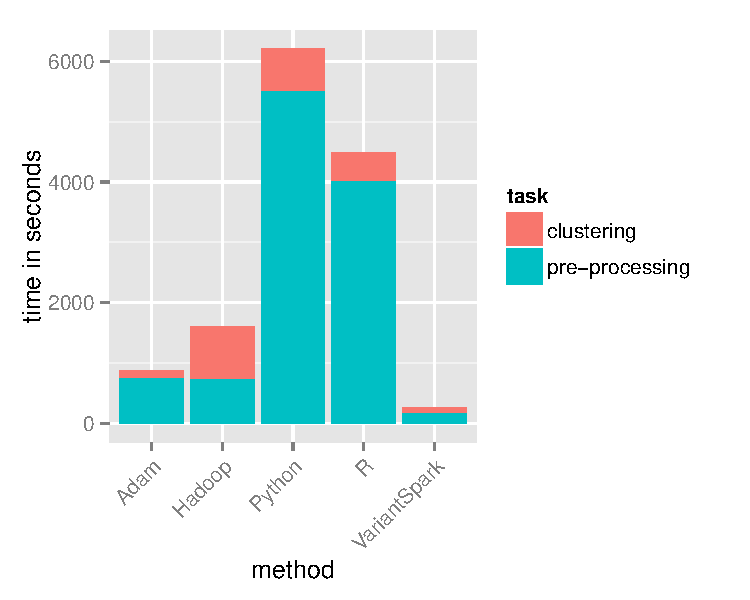
\includegraphics[type=pdf,ext=.pdf,read=.pdf, scale=0.45]{images/Resources}
  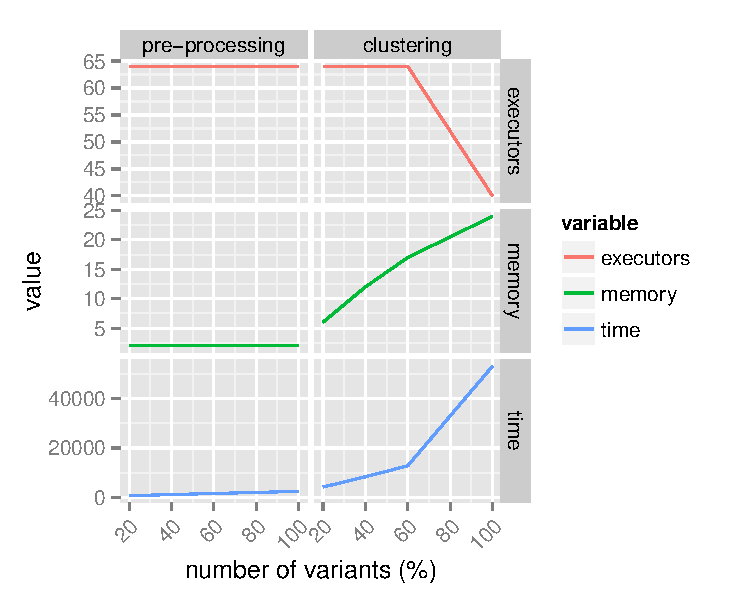
\includegraphics[type=pdf,ext=.pdf,read=.pdf, scale=0.45]{images/Scaling}
  \caption{\csentence{Comparison of method and genome-wide scaling experiment.}
      {\bf Left} Runtime is given in seconds with 32 GB of memory on 8 threads (except for the pre-processing in R and Python where this was not supported). 
      {\bf Right} Scaling from 20\% to 100\% of variants in the genome with maximal number of executors and lowest possible memory assignment.}
      \end{figure}

%Hadoop
%1. Map
%The mapper converts each line of the VCF file into a preliminary key-value pair, where the Key is the byte-position of the first character thereby functioning as a proxy for the genomic location (variant ID), and the Value is a string of the line. From this, the key-value pairs for the individual genotypes are created by extracting the variant from each sample as the new Value. The new key is a tuple consisting of the primary key, which is the individual ID (position of the parsed variants), and the variant ID as the secondary key.
%The MapReduce partitioner uses custom Collect/sort functions to collect the tuples by their primary key (individual ID) and distributes them between nodes. The data is sorted by secondary key (variant ID)
%2. Reduce
%This data is input to the Reducers, which store the variants for each individual to a sparse vector with the Key as the individual ID and the value as the variant vector.
%
%Spark
%1. The lines from the VCF file(s) are parsed independently by worker nodes, where each line is zipped with the heading from the VCF file resulting in tuples of individual ID and the variant. 
%2. These arrays are each zipped again with the unique, sequential index (the Variant ID) resulting in tuples (essentially key/value pairs) of Variant IDs (?key?) and the array of tuples from step 1 (?value?).
%3. The flatmap function restructures the data into Individual ID (?key?) and tuples with Variant ID and the Variant (?value?).
%4. These tuples are grouped by the Individual ID, collecting all Variant ID and Variant tuples, and non-zero variants are saved as a sparse vector.
\begin{figure}[h!]
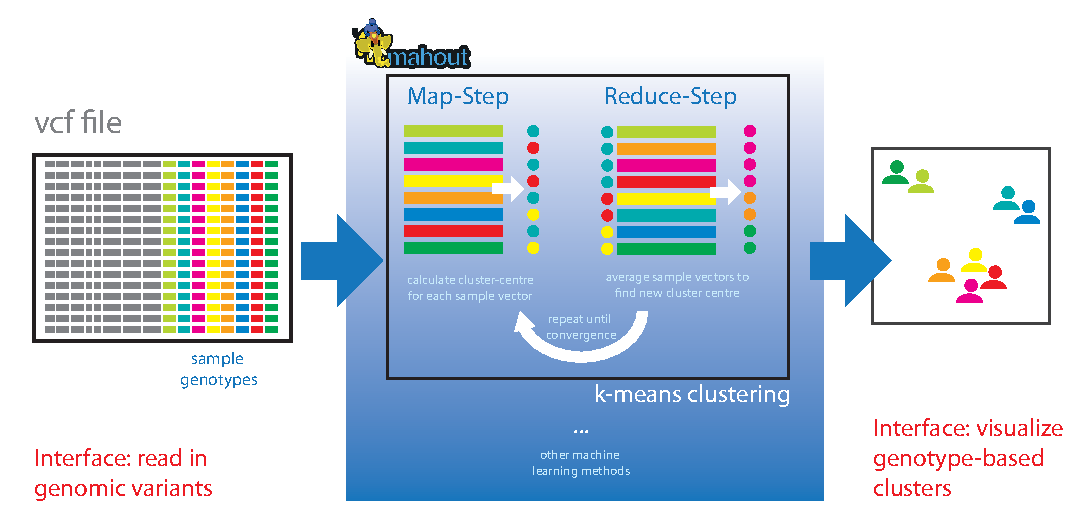
\includegraphics[type=pdf,ext=.pdf,read=.pdf, scale=0.25]{signature}
  \caption{\csentence{Schematic of the Hadoop and Spark implementation.} The image shows the conceptual differences in the steps necessary to convert variants in VCF to a data structure readable by Mahout and MLlib, respectively.}
      \end{figure}

\begin{figure}[h!]
  \caption{\csentence{Sample figure title.}
      Figure legend text.}
      \end{figure}

%%%%%%%%%%%%%%%%%%%%%%%%%%%%%%%%%%%
%%                               %%
%% Tables                        %%
%%                               %%
%%%%%%%%%%%%%%%%%%%%%%%%%%%%%%%%%%%

%% Use of \listoftables is discouraged.
%%
\section*{Tables}
\label{fivewaycomparison}
\begin{table}[h!]
\caption{The resources consumption of the six compared methods as well as the accuracy measured as \ARI{} on chromosome 22.}
      \begin{tabular}{|c|ccc|ccc|c|c|}
        \hline
           Tool &  \multicolumn{3}{ c |}{Pre-processing} & \multicolumn{3}{ c |}{Clustering} & Accuracy \\
& threads & memory & time  &threads & memory & time  & \\
  \hline
\variantSpark{}	& 8	& 32	& 2min 58sec	& 8	& 32	& 1min 20sec	& 0.84	\\ 
{\sc ADAM}		& 8	& 32	& 12min 48sec	& 8	& 32	& 1min 52sec	& 0.84	\\
Hadoop		& 8	& 32	& 14min 22sec	& 8	& 32	& 14min 23sec	& 0.84	\\
R			& 1	& 32	& 67min		& 8	& 32	& 7min 25sec	& 0.84	\\
Python		& 1	& 32	& 92min		& 8	& 32	& 11min 29sec	& 0.84	\\
{\sc Admixture}	& 1	& 32	& 10min 8sec	& 8	& 32 & 8min 19sec	& 0.25	\\
  \hline
      \end{tabular}
\end{table}

\label{scalingcomparison}
\begin{table}[h!]
\caption{The resources consumption on different subsets of the entire autosome (chromosomes 1-22). Memory specified is the memory allocated to each executor.}
      \begin{tabular}{|c|ccc|ccc|c|c|}
        \hline
           Portion &  \multicolumn{3}{ c |}{Pre-processing} & \multicolumn{3}{ c |}{Clustering}  \\
& executors & memory & time  & executors & memory & time \\
  \hline
20\%		& 64	& 2	& 11min 53sec	& 64	& 6	& 1hr 10min	\\
40\%		& 64	& 2	& 19min 9sec	& 64	& 12	& 2hr 19min	\\
60\%		& 64	& 2	& 26min 34sec	& 64	& 17	& 3hr 33min	\\
100\%	& 64	& 2	& 40min 48sec	& 40	& 24	& 14hr 44min	\\
  \hline
      \end{tabular}
\end{table}

%%%%%%%%%%%%%%%%%%%%%%%%%%%%%%%%%%%
%%                               %%
%% Additional Files              %%
%%                               %%
%%%%%%%%%%%%%%%%%%%%%%%%%%%%%%%%%%%

\section*{Additional Files}
  \subsection*{Additional file 1 --- Sample additional file title}
    Additional file descriptions text (including details of how to
    view the file, if it is in a non-standard format or the file extension).  This might
    refer to a multi-page table or a figure.

  \subsection*{Additional file 2 --- Sample additional file title}
    Additional file descriptions text.


\end{backmatter}
\end{document}
